\documentclass[12pt,letterpaper]{article}
\usepackage{fullpage}
\usepackage[top=2cm, bottom=4.5cm, left=2.5cm, right=2.5cm]{geometry}
\usepackage{amsmath,amsthm,amsfonts,amssymb,amscd}
\usepackage{lastpage}
\usepackage{enumerate}
\usepackage{fancyhdr}
\usepackage{mathrsfs}
\usepackage{xcolor}
\usepackage{graphicx}
\usepackage{listings}
\usepackage{hyperref}

\lstset{frame=lrb,xleftmargin=\fboxsep,xrightmargin=-\fboxsep}
\hypersetup{%
  colorlinks=true,
  linkcolor=blue,
  linkbordercolor={0 0 1}
}
 
\renewcommand\lstlistingname{Output}
\renewcommand\lstlistlistingname{Algorithms}
\def\lstlistingautorefname{Alg.}

\lstdefinestyle{Python}{
    language        = R,
    frame           = lines, 
    basicstyle      = \footnotesize,
    keywordstyle    = \color{blue},
    stringstyle     = \color{green},
    commentstyle    = \color{red}\ttfamily
}

\setlength{\parindent}{0.0in}
\setlength{\parskip}{0.05in}

% Edit these as appropriate
\newcommand\course{Statistical Methods in Research}
\newcommand\hwnumber{1}                  

\newcommand\NetIDb{Akshit Tandon - 1792038}      

\pagestyle{fancyplain}
\headheight 35pt
\lhead{\NetIDa}
\lhead{\NetIDa\\\NetIDb}                 % <-- Comment this line out for problem sets (make sure you are person #1)
\chead{\textbf{\Large Assignment \hwnumber}}
\rhead{\course}
\lfoot{}
\cfoot{}
\rfoot{\small\thepage}
\headsep 1.5em
\begin{document}
{\Large {\textbf{Question 1}}}\\

\textbf{(a)}
Mean = 292.3922,
    		  Median = 249\\
              Since, the mean is greater than the median. The distribution is right skewed.\\
   \begin{figure}[!h]
   \centering
    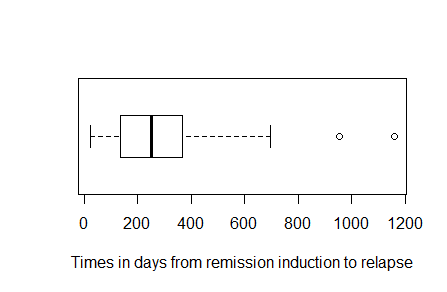
\includegraphics[width=0.5\linewidth]{Rplot.png}
    \caption{BoxPlot}
    \end{figure}
     \begin{lstlisting}[label=R Code,caption=Q1(a) R Code Output]
> boxplot(myData, outline = TRUE,horizontal = TRUE, xlab =
+         "Times in days from remission induction to relapse")
> boxplot.stats(myData)
$stats
[1]  24.0 135.5 249.0 367.0 697.0

$n
[1] 51

$conf
[1] 197.782 300.218

$out
[1]  955 1160
\end{lstlisting}
 
 {(\textbf{b})} There could be or could not be any outliers in the dataset. Sometimes uneven values are due to something significant and scientific and sometimes they are just error.\\ 
 You can drop the outliers if you are very confident that these value are out of scope or if you can verify the results by doing the experiment again.\\
\\ 
{(\textbf{c})}Percent of  patients  in remission for less than one year:  74.50\\
\\
{\Large {\textbf{Question 2}}}\\

{(\textbf{a})} Probability Distribution of Y
\begin{center}
 \begin{tabular}{||c | c ||} 
 \hline
 Y & PD \\ [0.5ex] 
 \hline
 0 & 150000-1031/150000 \\ 
 \hline
 50,000 & 1/150000 \\ 
 \hline
 10,000 & 5/150000 \\
 \hline
 1000 & 25/150000 \\
 \hline
 10 & 1000/150000 \\[1ex] 
 
 \hline
\end{tabular}
\end{center}

{(\textbf{b})} 
{\displaystyle \operatorname {E} [X]=\sum _{i=1}^{k}x_{i}\,p_{i}=x_{1}p_{1}+x_{2}p_{2}+\cdots +x_{k}p_{k}.}
{\displaystyle \operatorname {E} [X] =  \ 0.9}

{(\textbf{c})} Mean Expected Value =$0.9$ and the ticket cost is 1. So there will be a loss of  \$0.10.Hence, it is not worthwhile to purchase the ticket.\\

{(\textbf{d})} 

Standard \ Deviation = 	142.00
\begin{lstlisting}[label=R Code,caption=Q4(a) R Code Output]
      
> vec <- c(50000,rep(10000, each = 5),
rep(1000,each = 25),rep(10,each = 1000),
+          rep(0,each = 150000-1031))
> sd(vec)
[1] 142.0094
\end{lstlisting}
{\Large \textbf{Question 3}}\\
(Assuming sample is normally distributed.)\\

{(\textbf{a})} The target population are the  adults who have experienced feeling of depression or sadness.

{(\textbf{b})} Probability that your sample will have 12 or more people
with these feelings = 0.017
\begin{lstlisting}[label=R Code,caption=Q3(b) R Code Output]
> p_hat = 12/68
> p <- 0.10
> p
[1] 0.1
> n <- 68
> n
[1] 68
> SD <- sqrt(p*(1-p)/n)
> SD
[1] 0.03638034
> z_score = (p_hat - p)/SD
> ans_a = pnorm(z_score,lower.tail = FALSE)
> ans_a
[1] 0.01777771
          
\end{lstlisting}

{(\textbf{c})} There is a 1.7\% chance that in my sample of 68 people, more than 12 people will have such feelings. \\

{(\textbf{d})} Probability that the sample percentage will differ from this by more than 5 percent  = 0.16\\

\begin{lstlisting}[label=R Code,caption=Q3(d) R Code Output]
      
> z_score_1 = (0.15 - 0.10)/SD
> z_score_1
[1] 1.374369
> z_score_2 = (0.05-0.10)/SD
> z_score_2
[1] -1.374369
> ans_d = pnorm(z_score_1,lower.tail = FALSE) + 
+         pnorm(z_score_2)
> ans_d
[1] 0.1693273
          
\end{lstlisting}

{\Large \textbf{Question 4}}

{\textbf{(a)}} \\
$H0$ : Mean = \$14200\\
            $H1$: Mean \ne \$14200 
            \\
            Population\ Mean = 14200\\
            Sample\ Mean = 15300\\
            Standard\ Error = 2600/sqrt(75) = 300.22\\
            t\ value = 3.66\\
           -1.99 \leq Alpha\ Range \leq 1.99\\
            Level\ of\ Significance = 0.05\\
            
            Result: Since, t value  does  not  lie  in the critical range, 
            we reject the NULL hypothesis at 0.05 level of significance\\ 
             
           \begin{lstlisting}[label=R Code,caption=Q4(a) R Code Output]
      
> pop_mean = 14200
> sample_mean = 15300
> pop_sd = 2600
> givenAlpha = 0.05
> mySampleSize = 75
> se <- pop_sd/sqrt(mySampleSize)
> 
> t_value_stat = (sample_mean - pop_mean)/se
> t_value_stat
[1] 3.663954
> alpha_range = qt(1-givenAlpha/2,df = mySampleSize-1)
> critical_range = c(-alpha_range,alpha_range)
> critical_range
[1] -1.992543  1.992543
          
\end{lstlisting}

{(\textbf{b})}  \\
Confidence\ Level = 99 \%\\
Critical\ Value = 2.37 \\
Margin\ Error = Standard Error * Critical \ Value = 713.86 \\
Confidence\ Interval = Sample Mean +- Margin Error\\
Confidence\ Interval : 14586 \leq Sample Mean \leq 16014\\

Result : We are 99\% confident that the sample mean will lie between 14586 and 16014\\
\\

\begin{lstlisting}[label=R Code,caption=Q4(b) R Code Output]
      
> val = qt(0.99,df = 74)
> val
[1] 2.377802
> marginError <- val * se
> marginError
[1] 713.8688
> confidenceInterval = c(sample_mean - marginError , sample_mean 
+ marginError)
> confidenceInterval
[1] 14586.13 16013.87
          
\end{lstlisting}
\\
{(\textbf{c})}
\begin{figure}[!h]
   \centering
    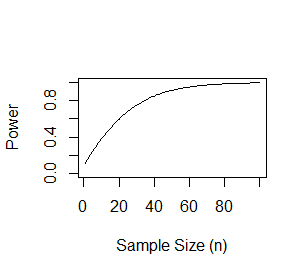
\includegraphics[width=0.5\linewidth]{PC.png}
    \caption{Power Curve}
    \end{figure}

\begin{lstlisting}[label=R Code,caption=Q4(c) R Code Output]
> power_curve <- function(n = 75,alpha = 0.05,H0 = 14200,H1 = 15300,
+                         sig = 2600)
+ {
+   zee <- qnorm(p = alpha,mean = 0,sd = 1,lower.tail = FALSE)
+   cr <- zee * (sig/sqrt(n)) + H0;
+   power <- pnorm(q = cr,mean = H1,sd = sig/sqrt(n),
lower.tail = FALSE)
+   power
+ }
> power_curve()
[1] 0.9782616
> mycurve1 <- lapply(X = 1:100, FUN = power_curve,alpha = .05
+                    ,H0 = 14200,H1 = 15300,sig = 2600)
> plot(x = 1:100,y = mycurve1,type = "line",
xlab = "Sample Size (n)", ylim = c(0,1),
+      ylab = "Power")
\end{lstlisting}
{\Large \textbf{Question 5}} \\
\\
{\textbf{(a)}} \\
$H0$ : Mean =\ 2700\\
	  $H1$: Mean \ne\ $2700$
	  \\
	  Population\ Mean = 2600\\
	  Sample \Mean = 2620\\
	  Standard \ Error = 450/sqrt(36) = 75\\
	  t \ value = -1.06\\
	   -2.03 \leq Alpha\ Range \leq 2.03\\
	  Level \ of \ Significance = 0.05\\
      
	  Result: Since, t value is in range of critical Values,
      we do not reject the NULL hypothesis.\\
      \\
      
      \begin{lstlisting}[label=R Code,caption=Q5(a) R Code Output]
      
> given_pop_mean = 2700
> given_sample_mean = 2620
> given_pop_sd = 450
> alpha = 0.05
> size = 36
> standard_e = given_pop_sd/sqrt(size)
> t_value = (given_sample_mean - given_pop_mean)/standard_e
> t_value
[1] -1.066667
> d_range = qt(1-alpha/2,df = size-1)
> f_range = c(-d_range,d_range)
> f_range
[1] -2.030108  2.030108
          
\end{lstlisting}
{(\textbf{b})}(Assuming sample is normally distributed.)\\
Power = \ 0.26\\
\begin{lstlisting}[label=R Code,caption=Q5(b) R Code Output]
> lower_bound = qnorm(alpha/2,mean = 2700,sd = standard_e)
> lower_bound
[1] 2553.003
> upper_bound = qnorm(alpha/2,mean = 2700,
sd = standard_e, lower.tail = FALSE)
> upper_bound
[1] 2846.997
> given_mean = 2600
> z_lower = (lower_bound - given_mean)/standard_e
> z_lower
[1] -0.6266307
> z_upper = (upper_bound - given_mean)/standard_e
> z_upper
[1] 3.293297
> p_lower = pnorm(z_lower)
> p_lower
[1] 0.2654507
> p_upper = pnorm(z_upper,lower.tail = FALSE)
> p_upper
[1] 0.0004950985
> power = p_lower + p_upper
> power
[1] 0.2659458
\end{lstlisting}
\end{document}